\documentclass[11pt]{scrartcl}

\usepackage{amsmath}
\usepackage{float}
\usepackage{tikz}
\usepackage{cleveref}
\renewcommand{\rmdefault}{ppl}% rm
\linespread{1.05}
\usepackage[scaled]{helvet}
\usepackage{courier}
\normalfont
\usepackage[T1]{fontenc}
\usepackage{textcomp}

\usetikzlibrary{shapes,arrows,positioning}

\tikzset{block/.style = {draw, rectangle, minimum height = 2em, minimum width = 3em},
         prod/.style = {draw, circle},
         sync/.style = {draw, rectangle, draw=black!50, fill=black!20, thick, minimum height =0.7cm},
         input/.style = {coordinate},
         output/.style = {coordinate},
}

\begin{document}

\title{Bluestein's Algorithm}
\subtitle{rocFFT design document}
\date{\vspace{-5ex}}

\maketitle

\section{Summary}
This document reviews Bluestein's algorithm and describe its current implementation in rocFFT. A new implementation of Bluestein's algorithm is proposed. The proposed implementation may provide several benefits, including improved performance and the ability to reuse the design to perform fast convolutions without any major modifications.

\section{Background and Notation}

\subsection{Discrete Fourier Transform}
Let $ \mathbf{X} = \mathcal{F}\left\{ \mathbf{x} \right\}$ denote the discrete Fourier transform (DFT) of $\mathbf{x}$, which maps an $N$-length input sequence $\mathbf{x} = \begin{bmatrix} x_0 &  \cdots & x_{N-1} \end{bmatrix}$ into an $N$-length output sequence $\mathbf{X} = \begin{bmatrix} X_0 & \cdots & X_{N-1} \end{bmatrix}$ with
\begin{equation}
X_k = \sum_{n=0}^{N-1}{x_n e^{-\frac{2 \pi \jmath}{N}nk}}, \qquad k = 0, \ \ldots, \ N-1.
\label{eq:dft}
\end{equation}
Conversely, let $\mathbf{x} = \mathcal{F}^{-1}\left\{ \mathbf{X} \right\}$ denote the inverse DFT, which maps the sequence $\mathbf{X}$ into sequence $\mathbf{x}$ as follows
\begin{equation}
x_k = \frac{1}{N}\sum_{n=0}^{N-1}{X_n e^{\frac{2 \pi \jmath}{N}nk}}, \qquad k = 0, \ \ldots, \ N-1.
\label{eq:idft}
\end{equation}
In Bluestein's algorithm, the following identity is considered for the DFT computation
\begin{equation}
nk = \frac{-(k-n)^2}{2} + \frac{n^2}{2} + \frac{k^2}{2}.
\label{eq:index_identity}	
\end{equation}
For example, substituting \labelcref{eq:index_identity} into \labelcref{eq:dft}, the DFT can then be expressed as

\begin{equation}
X_k = e^{-\frac{\pi \jmath}{N}k^2} \sum_{n=0}^{N-1}{\left( x_n e^{-\frac{\pi \jmath}{N}n^2} \right) e^{\frac{\pi \jmath}{N}  (k-n)^2}{}}, \qquad k = 0, \ \ldots, \ N-1.
\label{eq:bluestein_dft}	
\end{equation}

\subsection{Chirp}
Bluestein's algorithm is frequently used to compute the DFT, but it can also be used to compute the more general z-transform. This transform is similar to \labelcref{eq:dft} with the difference that the term $e^{-\frac{2\pi \jmath}{N}}$ is replaced by $z$, where $z$ is an arbitrary complex number. 

Let $\mathbf{c} = \begin{bmatrix} c_0 & \cdots & c_{N-1} \end{bmatrix}$ denote an $N$ length sequence of the form
\begin{equation}
c_n = e^{\frac{\pi \jmath}{N}n^2}, \qquad n = 0, \ \ldots, \ N-1.
\label{eq:chirp}
\end{equation}
The sequence $\mathbf{c}$, which is present in \labelcref{eq:bluestein_dft}, is also known as \emph{chirp} because it defines a complex sinusoid of linearly increasing frequency. Bluestein's algorithm is also known as the chirp z-transform for this reason.

\subsection{Convolution}

Now let $\left(\mathbf{a} \ast \mathbf{b}\right)_k$ for $k = 0, \ \ldots, \ M-1$ denote the convolution of two $M$-length input sequences $\mathbf{a} = \begin{bmatrix} a_0 & \cdots a_{M-1} \end{bmatrix}$ and $\mathbf{b} = \begin{bmatrix} b_0 & \cdots b_{M-1} \end{bmatrix} $ with

\begin{equation}
\left(\mathbf{a} \ast \mathbf{b} \right)_k = \sum_{m=0}^{M-1}a_m b_{k-m}, \qquad k = 0, \ \ldots, \ M-1.
\label{eq:convolution_definition}	
\end{equation}
The DFT in \labelcref{eq:bluestein_dft} can be expressed in terms of the convolution sum in \labelcref{eq:convolution_definition} as
\begin{equation}
X_k = b_k^{-1} \sum_{m=0}^{M-1}{a_m b_{k-m}}, \qquad k = 0, \ \ldots, \ M-1,
\label{eq:bluestein_convolution}
\end{equation}
with $M=N$, $a_m = x_m / c_m$, and $b_m = c_m$ for $m = 0, \ \ldots, \ M-1$.

From the convolution theorem we know that, under suitable conditions, the convolution sum in \labelcref{eq:convolution_definition} can be evaluated by computing the point-wise product of the DFTs of $\mathbf{a}$ and $\mathbf{b}$ and taking the inverse DFT of the product
\begin{equation}
\left(\mathbf{a} \ast \mathbf{b} \right) = \mathcal{F}^{-1}\left\{ \mathcal{F}\left\{ \mathbf{a} \right\} \cdot \mathcal{F}\left\{ \mathbf{b} \right\} \right\}. \label{eq:convolution_dft}	
\end{equation}
Note, however, that \labelcref{eq:convolution_dft} cannot be used to directly evaluate \labelcref{eq:bluestein_dft} under the values of $M$, $a_m$ and $b_m$ provided.  

\subsection{Zero padding}
Consider instead that the DFT in \labelcref{eq:bluestein_convolution} is evaluated with
\begin{equation}
M \geq 2N-1
\label{eq:bluestein_length_requirement}
\end{equation}
and the sequences $\mathbf{a}$ and $\mathbf{b}$ are zero-padded as follows
\begin{align}
a_m &= \begin{cases} x_n / c_n& \text{for $n = 0, \ \ldots, \ N-1$},\\ 0 & \text{otherwise} \end{cases} \label{eq:first_zero_pad} \\
b_m &= \begin{cases} c_n& \qquad \text{for $n = 0, \ \ldots, \ N-1$ \ and $n = M - N + 1, \ \ldots, \ M - 1$},\\ 0 & \qquad \text{otherwise.} \end{cases}
\label{eq:second_zero_pad}
\end{align}
In Bluestein's algorithm, the conditions in \labelcref{eq:bluestein_length_requirement,eq:first_zero_pad,eq:second_zero_pad} ensure that the convolution theorem holds and, therefore, \labelcref{eq:convolution_dft} can be employed to evaluate \labelcref{eq:bluestein_dft}.


\section{Implementation} 
Based on the conditions in \labelcref{eq:bluestein_length_requirement,eq:first_zero_pad,eq:second_zero_pad} and the convolution theorem in \labelcref{eq:convolution_dft}, the DFT can be computed as follows in Bluestein's algorithm
\begin{equation}
X_k = b_k^{-1} \mathcal{F}^{-1}\left\{ \mathcal{F}\left\{ \mathbf{a} \right\} \cdot \mathcal{F}\left\{ \mathbf{b} \right\} \right\}, \qquad k = 0, \ \ldots, \ N-1.
\label{eq:bluestein_final}
\end{equation}
There are quite a few operations involved in this computation. More specifically, computation of the chirp sequence, two $N$-length plus one $M$-length point-wise multiplications, zero-padding of two $M$-length sequences, and two forward DFTs of length $M$ plus an inverse DFT also of length $M$. 

The main reason for using Bluestein's algorithm is that it applies for the DFT computation of any input length $N$, including prime lengths. When a fast Fourier transform (FFT) algorithm is used to compute the DFT, such as Stockham or Cooley-Tukey, it usually provides optimized length support via a given radix or combination of radices, e.g., $N = 2, \ 3, \ 5, \ 25 \times 2, \ 16 \times 9$, and so on. Considering that the DFTs in \labelcref{eq:bluestein_final} can be carried out with any length satisfying \labelcref{eq:bluestein_length_requirement}, a suitably chosen value of $M$ can be used to compute the  convolution via an FFT with existing radix support. However, it should be mentioned that the computation in \labelcref{eq:bluestein_final} is much slower than directly computing \labelcref{eq:dft} via the FFT with a supported length, even though both computations posses the same complexity of $O(N \log N)$.

An illustration of the steps required for Bluestein's algorithm is given in \Cref{fig:bluestein_diagram}. 

\begin{figure}[H]
\centering
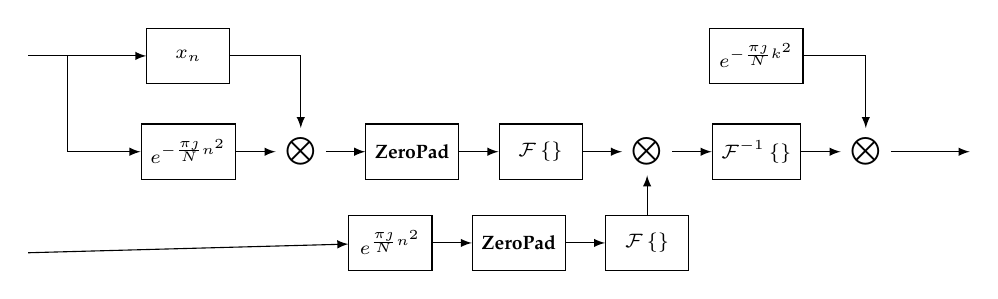
\begin{tikzpicture}[auto, node distance = .5cm]
  \node[block, font = \scriptsize] (CHIRP1)  {$e^{-\frac{\pi \jmath}{N}n^2}$};
  \node[right = of CHIRP1] (HAD1)  {$\bigotimes$};
  \node[block, above = of CHIRP1,  font = \scriptsize] (IN)  {$x_n$};
  
  \node[input, left = of IN, name = coor1] {};
  \node[input, left = of coor1, name = coor2] {};
  \node[input, below = of coor2, name = coor3] {};
  \node[input, left = of coor2, name = in] {};
  
  \node[input, below = of in, name = coor4] {};
  
  \node[input, below = of coor4, name = coor5] {};
  \node[input, below = of coor5, name = coor6] {};
  \node[input, below = of coor6, name = coor7] {};
  \node[input, below = of coor7, name = coor8] {};
  \node[input, below = of coor8, name = coor9] {};
  
  \node[block, right = of HAD1, font = \scriptsize] (ZPAD1)  {$\textbf{ZeroPad}$};
  \node[block, right = of ZPAD1, font = \scriptsize] (FFT1)  {$\mathcal{F}\left\{ \right\}$};

  \node[right = of FFT1] (HAD2)  {$\bigotimes$};
   
  \node[block, below = of HAD2, font = \scriptsize] (FFT2)  {$\mathcal{F}\left\{ \right\}$};
  
  \node[block, left = of FFT2, font = \scriptsize] (ZPAD2)  {$\textbf{ZeroPad}$};  
  \node[block, left = of ZPAD2, font = \scriptsize] (CHIRP2)  {$e^{\frac{\pi \jmath}{N}n^2}$};

  
  \node[block, right = of HAD2, font = \scriptsize] (IFFT)  {$\mathcal{F}^{-1}\left\{ \right\}$};
 
  \node[right = of IFFT] (HAD3)  {$\bigotimes$};
  
  \node[block, above = of IFFT, font = \scriptsize] (CHIRP3)  {$e^{-\frac{\pi \jmath}{N}k^2}$};

  \node[output, right = of HAD3, name = coord10] {};  
  \node[output, right = of coord10, name = out] {};

  \draw[-latex] (in) -- (IN);  

  \draw[-latex] (IN) -| (HAD1);
  \draw[-latex] (coor2) |- (CHIRP1);  
  
  \draw[-latex] (coor8) -- (CHIRP2);  

  \draw[-latex] (CHIRP1) -- (HAD1);
  \draw[-latex] (HAD1) -- (ZPAD1);
  \draw[-latex] (ZPAD1) -- (FFT1);
  \draw[-latex] (FFT1) -- (HAD2);
  
  
  \draw[-latex] (CHIRP2) -- (ZPAD2);
  \draw[-latex] (ZPAD2) -- (FFT2);
  \draw[-latex] (FFT2) -- (HAD2);
  
  \draw[-latex] (HAD2) -- (IFFT);
  \draw[-latex] (IFFT) -- (HAD3);  
  \draw[-latex] (CHIRP3) -| (HAD3);  
  
  \draw[-latex] (HAD3) -- (out);    
  
\end{tikzpicture}
\caption{Diagram of computations involved in Bluestein's algorithm}
\label{fig:bluestein_diagram}
\end{figure}

A few observations can be made from the block diagram.  First, it can be seen that there are no direct dependencies between the two branches that compute $\mathcal{F}\left\{ \mathbf{a} \right\}$ and $\mathcal{F}\left\{ \mathbf{b} \right\}$ and, therefore, parallelization may be leveraged to speed-up the computations and perform the two sequence of operations independently. Second, it can further be seen that the chirp sequence is used multiple times throughout the diagram. Reutilizing the computed chirp sequence across the operations where possible may also be advantageous. Third, there are quite a few number of operations in the diagram, and it is, therefore, often preferable to put together these operations into as little as possible device kernels, due to the overhead of kernel launch.

\subsection{Current kernel configuration}

The current configuration for Bluestein's algorithm in rocFFT is illustrated in \Cref{fig:kernel_configuration_current}. 

\begin{figure}[H]
\centering
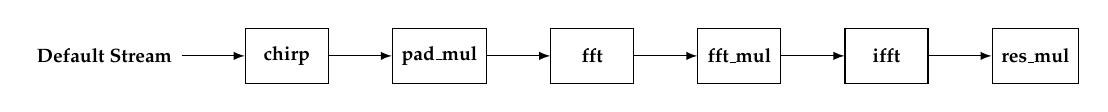
\begin{tikzpicture}[auto, node distance = .8cm]

  
  \node[block, font = \scriptsize] (chirp)  {$\textbf{chirp}$};
  \node[left = of chirp,font = \scriptsize] (in){$\textbf{Default Stream}$};
  \node[block, right = of chirp, font = \scriptsize] (pad_mul)  {$\textbf{pad\_mul}$};
  \node[block, right = of pad_mul, font = \scriptsize] (fft)  {$\textbf{fft}$};
  \node[block, right = of fft, font = \scriptsize] (fft_mul)  {$\textbf{fft\_mul}$};
  \node[block, right = of fft_mul, font = \scriptsize] (ifft)  {$\textbf{ifft}$};
  \node[block, right = of ifft, font = \scriptsize] (res_mul)  {$\textbf{res\_mul}$};

  \draw[-latex] (in) -- (chirp);  
  \draw[-latex] (chirp) -- (pad_mul);
  \draw[-latex] (pad_mul) -- (fft);
  \draw[-latex] (fft) -- (fft_mul);  
  \draw[-latex] (fft_mul) -- (ifft);    
  \draw[-latex] (ifft) -- (res_mul);      
  
\end{tikzpicture}
\caption{Current configuration of device kernels for Bluestein's algorithm}
\label{fig:kernel_configuration_current}
\end{figure}

As can be seen from the diagram, Bluestein's algorithm is performed with (at least) six kernels in a single device stream. When the input length $N$ is above a certain threshold and the Stockham FFT kernels no longer fit into shared memory, a hierarchical approach is utilized where the large FFT is split into multiple smaller FFT kernels that fit into shared memory for improved performance. The \emph{fft} and \emph{ifft} kernels in the diagram are, therefore, executed in at least two separate kernels.

The chirp sequence is computed in a single \emph{chirp} kernel, and the sequence is reutilized at later stages via a temporary device buffer. The two forward DFTs are joined together in (at least) one \emph{fft} kernel. This is possible because the padded sequences $\mathbf{a}$ and $\mathbf{b}$ are contiguous in the temporary device buffer, thus allowing for a single kernel to perform the two operations. The inverse FFT operation requires a separate \emph{ifft} kernel. Similarly, the three point-wise multiplications are carried out with separate kernels, \emph{pad\_mul}, \emph{fft\_mul}, and \emph{res\_mul}.

\subsection{Proposed kernel configuration}
The proposed kernel configuration for Bluestein's algorithm is based on the following three design choices:
\begin{enumerate}
\item Leverage parallelism in the algorithm stages.
\item Use the convolution as a building block for the algorithm.
\item Minimize the number of device kernels.
\end{enumerate}

As shown in \Cref{fig:bluestein_diagram}, there is opportunity for parallelism in Bluestein's algorithm since the computation of the two sequences $\mathbf{a}$ and $\mathbf{b}$ and their respective forward DFTs are independent from each other. This inherent parallelism is leveraged in the proposed fast convolution building block in \Cref{fig:kernel_configuration_convolution_proposed}.

\begin{figure}[H]
\centering
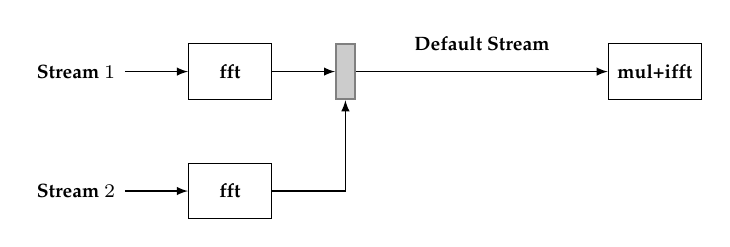
\begin{tikzpicture}[auto, node distance = .8cm]

  \node[block, font = \scriptsize] (fft1)  {$\textbf{fft}$};
  \node[left = of fft1,font = \scriptsize] (in1){$\textbf{Stream } 1$};
  \node[block, below = of fft1, font = \scriptsize] (fft2)  {$\textbf{fft}$};
  \node[left = of fft2,font = \scriptsize] (in2){$\textbf{Stream } 2$};
  \node[sync, right = of fft1, font = \scriptsize] (sync)  {$\textbf{}$};
  \node[output, right = of sync] (out1) {};
  \node[output, right = of out1] (out2) {};
  \node[output, right = of out2] (out3) {};
  \node[block, right = of out3, font = \scriptsize] (ifft)  {$\textbf{mul+ifft}$};
  \node[font = \scriptsize] at (3.2, .35) (ds){$\textbf{Default Stream}$};

  \draw[-latex] (in1) -- (fft1);  
  \draw[-latex] (in2) -- (fft2);  
  \draw[-latex] (fft1) -- (sync);
  \draw[-latex] (fft2) -| (sync);
  \draw[-latex] (sync) -- (ifft);
  
\end{tikzpicture}
\caption{Proposed configuration of device kernels for fast convolution}
\label{fig:kernel_configuration_convolution_proposed}
\end{figure}

In the proposed building block, two separate device streams are used to carry out the forward DFTs in the convolution theorem in \labelcref{eq:convolution_dft}. Since the input buffers in a (possibly?) future implementation of fast convolution in rocFFT will unlikely be contiguous, as they may be implemented with different offsets and stride requirements, it is, therefore, unlikely that the two forward DFTs can be joined into a single operation. The convolution building block thus leverage the inherent parallelism of the separate streams. A drawback of this approach is that a synchronization step is required after the forward DFTs stage. This is denoted by the thin solid rectangle in the diagram. Lastly, following the design principle of minimizing the number of device kernels, the point-wise multiplication and inverse DFT are fused into a single device kernel.

Based upon the fast convolution building block in \Cref{fig:kernel_configuration_convolution_proposed}, the proposed kernel configuration for Bluestein's algorithm is illustrated in \Cref{fig:kernel_configuration_proposed}.

\begin{figure}[H]
\centering
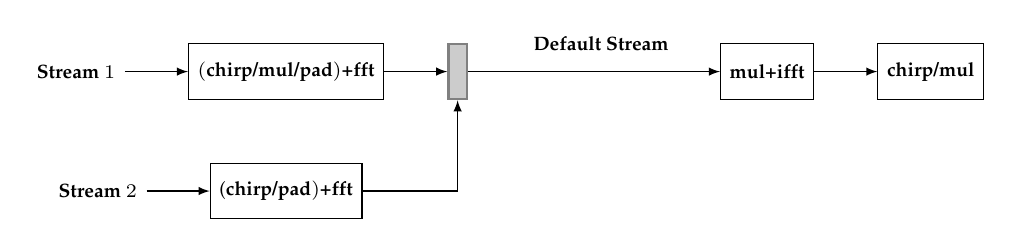
\begin{tikzpicture}[auto, node distance = .8cm]

  \node[block, font = \scriptsize] (fft1)  {$(\textbf{chirp/mul/pad})\textbf{+fft}$};
  \node[left = of fft1,font = \scriptsize] (in1){$\textbf{Stream } 1$};
  \node[block, below = of fft1, font = \scriptsize] (fft2)  {($\textbf{chirp/pad})\textbf{+fft}$};
  \node[left = of fft2,font = \scriptsize] (in2){$\textbf{Stream } 2$};
  \node[sync, right = of fft1, font = \scriptsize] (sync)  {$\textbf{}$};
  \node[output, right = of sync] (out1) {};
  \node[output, right = of out1] (out2) {};
  \node[output, right = of out2] (out3) {};
  \node[block, right = of out3, font = \scriptsize] (ifft)  {$\textbf{mul+ifft}$};
  \node[block, right = of ifft, font = \scriptsize] (res)  {$\textbf{chirp/mul}$};
  \node[font = \scriptsize] at (4, .35) (ds){$\textbf{Default Stream}$};

  \draw[-latex] (in1) -- (fft1);  
  \draw[-latex] (in2) -- (fft2);  
  \draw[-latex] (fft1) -- (sync);
  \draw[-latex] (fft2) -| (sync);
  \draw[-latex] (sync) -- (ifft);
  \draw[-latex] (ifft) -- (res);
  
\end{tikzpicture}
\caption{Proposed configuration of device kernels for Bluestein's algorithm}
\label{fig:kernel_configuration_proposed}
\end{figure}

As can be seen from the diagram, the implementation of Bluestein's algorithm is quite similar to the convolution in \Cref{fig:kernel_configuration_convolution_proposed}. The main difference between the two is that the forward DFTs stage have fused operations in them, chirp + point-wise multiplication + padding in the first stream, and chirp + padding in the second stream. Additionally, after the fused point-wise multiplication + inverse DFT kernel, there is an additional chirp + point-wise multiplication kernel. In this last stage, the chirp may not need to be recomputed, but instead read from the temporary buffer which may already contain the chirp sequence from previous stages. An advantage of the proposed kernel configuration is that fast convolution and DFT via Bluestein's algorithm share many similarities. In other words, implementing Bluestein's algorithm may also get us fast convolution for free.


\end{document}
